\chapter{神经网络简介}

\citestyle{numbers}

\section{神经网络算法基础}
现代神经网络由多种不同类型的层组成,输入数据依次通过各个层被逐层处理,最终被分类,识别或者检测。在每一层中,神经元接收多个输入进行处理,然后通过连接将输出发送到下一层。神经元之间的连接,即所谓的突触,通常具有独立或者共享的权重。神经网络在图像处理,语音识别,语音合成,自然语言处理等领域有着非常广泛的应用。目前在图像处理应用最广泛的网络是卷积神经网络(convolutional neural networks,简称CNNs)和深度神经网络(deep neural networks,简称DNNs),它们由卷积层,池化层,归一化层,激活层和全连接层等组成。递归神经网络(recurrent neural networks,简称RNNs)是一类重要的机器学习技术,专门用于处理顺序数据序列和可变长度数据序列。RNNs在语音识别,自然语言处理,场景语义理解和时间序列分析等方面有着广泛的应用。其中应用最广泛,性能最高的两种类型的RNNs是长短时记忆网络(long short term memory,简称LSTM)和门控循环单元(gated recurrent unit,简称GRU)。下面将为大家介绍神经网络中集中常见的神经网络层类型。

\subsection{全连接层}
全连接层(fully connected layers)是神经网络算法中常见的一种层类型,主要用来将上一层提取的特征进行组合,综合以及分类,在整个神经网络中起到“分类器”的作用。全连接层的结构如图~\ref{fig:fc_layer}所示,输入层神经元为m个,输出层的神经元为n个,其中每一个输出神经元与所有输入神经元相连,其结构相当于n个m输入的感知机,因此全连接层也可以看成是感知机扩展。 
\begin{figure}
  \centering
  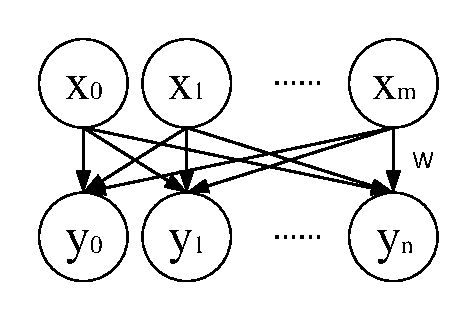
\includegraphics[width=0.5\columnwidth]{fc.pdf}
  \caption{\footnotesize 全连接层}
  \label{fig:fc_layer}
\end{figure}


全连接层的核心操作操作是矩阵向量乘积,
\begin{equation}
y=W*x+b
\end{equation}
其中$y$是输出神经元向量,$x$是输入神经元向量,$W$是权值矩阵,$b$是输出神经元的偏置向量。因此全连接层的本质是由一个特征空间线性变换到另一个特征空间,且目标空间的任一维都会收到源空间每一维的影响。由于每个输出神经元都要与输入神经元相连接,这样的话就会造成权值数量巨大,从而造成网络难以训练,并且会出现过拟合的情况。因此在CNN中,全连接层常出现在最后几层,用取于对前面设计提的特征做加权和。

\subsection{卷积层}
\begin{figure}[b]
  \centering
  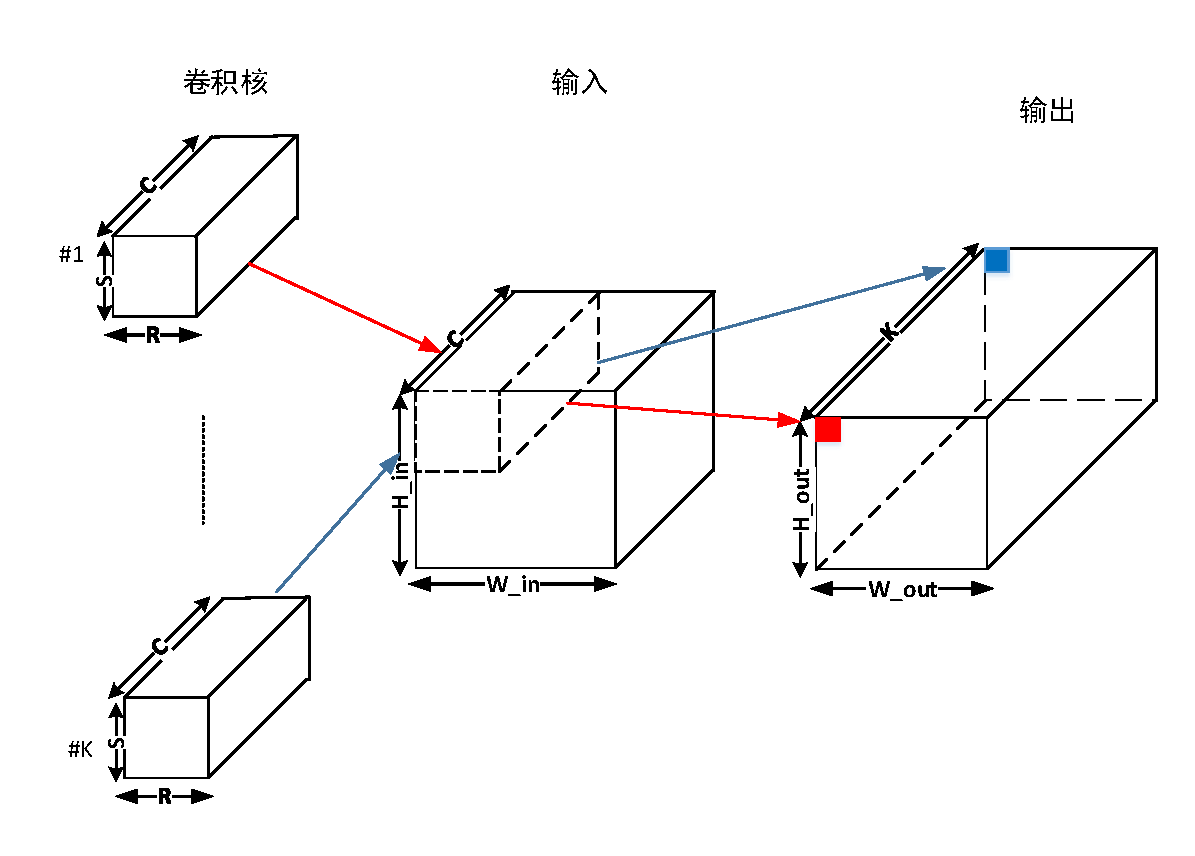
\includegraphics[width=0.8\columnwidth]{conv.pdf}
  \caption{\footnotesize 卷积层}
  \label{fig:conv_layer}
\end{figure}

卷积层(convolutional layers)是卷积神经网络的核心层,主要用于提取特征。卷积层受到生物学上感受野(Receptive Field)的机制而提出的。感受野主要是指听觉系统、本体感觉系统和视觉系统中神经元的一些性质。比如在视觉神经系统中,一个神经元的感受野是指视网膜上的特定区域,只有这个区域内的刺激才能够激活该神经元。在听觉系统中,对于语音则是某一时间戳后的时间段才能激活神经元。卷积层充分借鉴感受野的机制,神经元仅仅能够感受局部特征,而卷积核的大小直接限制感受野的大小,输出神经元只和周围一小块的输入神经元存在连接。局部连接的方法大大减少了卷积层中的权值数量。
卷积层采用了共享权值的方法进一步减少权值的数量,即同一输出特征图共享一组卷积核。同一个输出特征图像上的所有像素点是同一组卷积核在输入图像不同位置上提取到的图像特征,而这些图像特征具有相同意义。卷积层采用多组不同的卷积核对输入特征图进行卷积,从而获得多组输出特征图,即多组不同的图像特征。

卷积层的结构如图~\ref{fig:conv_layer}所示。卷积层的核心运算是二维滑动窗口卷积运算,即规模为$R\times S$的卷积核在规模为$W_{in}\times H_{in}$的输入特征图上滑动进行二维卷积,最终产生规模为$W_{out}\times H_{out}$的输出特征图。通常情况下,输入特征图不仅只有一个,而是由C个组成,即规模为$C\times W_{in}\times H_{in}$,因此我们对每个输入通道都施加一个卷积核,即使用规模为$C\times R\times S$的卷积核对输入进行卷积,最终获得一个输出特征图。当我们将采$K$组不同的卷积核作用于相同的输入特征图,将获得$K$个不同的输出特征图。最终,卷积层的输入规模为$C\times W_{in}\times H_{in}$,卷积核的规模为$K\times C\times R\times S$,输出规模为$K\times W_{out} \times W_{out}$。

\begin{lstlisting}[language=C, frame=single, basicstyle=\footnotesize, caption=六层卷积循环, label=list:convcode, captionpos=b]
for k=0 to K
    for w=0 to W
        for h=0 to H
            for c=0 to C
                for s=0 to S
                    for r=0 to R
                        out[k][w][h] += in[c][w*sw+r][h*sh+s] * filter[k][c][r][s]
\end{lstlisting}

卷积层的计算由K,C,R,S,W和H这六个变量形成嵌套循环完成,而且这六个变量的所有排列都是合法的。算法~\ref{list:convcode}展示了其中一种循环嵌套方式,我们可以用$N->W_{out}->H_{out}->C->S->R$来描述这种循环,其中$sw$和$sh$表示卷积操作的步长。不同的循环方式决定了数据的复用形式和数据流的方式,最终将影响神经网络加速器的设计~\cite{angshuman2017scnn}。

\subsection{池化层}
池化层(pooling layer)是神经网络中一个重要的层。池化层一般是在卷积层之后,对输入进行非线性降采样,常用的池化做法是对每个滤波器的输出求最大值,平均值,中位数等。
池化层的意义主要体现在两个方面:第一,池化层通过对特征图像进行降维操作,能够在保留显著特征的情况下,有效减少整个神经网络所需要的参数量和计算量。第二,池化层能够保证输入的平移不变性(translation invariant),这意味着即使图像的像素在邻域发生微小位移时,池化层的输出能够保持不变,从而增强神经网络的鲁棒性,由一定的抗扰动能力。常用的池化层包括最大池化层,平均池化层,ROI (Regions of interest)池化层.

最大池化层的基本思想是在一个特定的数据区域内选择一个最大值作为输出。其计算公式是
\begin{equation}
out_{x,y} = max(in_{x*sx,y*sy}:in_{x*sx+kx,y*sy+ky})
\end{equation}
其中$kx$和$ky$是池化窗口的大小,$sx$和$sy$是池化的步长。通常情况下池化窗口的大小与池化的步长相同,即池化操作的输入并不会重复。后来也出现了数据复用的池化,相邻池化窗口之间会有重叠区域,此时池化步长小于池化窗口的大小。


平均池化层的基本操作与最大池化层类似,它将一个特定的区域内的数据取算数平均作为输出,其计算公式是
\begin{equation}
out_{x,y}=mean(in_{x*sx,y*sy}:in_{x*sx+kx,y*sy+ky})
\end{equation}

ROI Pooling层主要是针对ROIs的池化操作,主要应用于物体检测领域的Fast RCNN和Faster RCNN网络中,它的特点是输入特征图尺寸不固定,但是输出特征图的尺寸固定。ROI Pooling的输入包含两部分,第一部分是特征图,在Fast RCNN中,它位于ROI Pooling之前;在Faster RCNN中,它是与RPN共享的那个特征图。第二部分是ROIS,在Fast RCNN中,指的是Selective Search的输出;在Faster RCNN中指的是RPN的输出,是一系列的矩阵候选框,每一个矩阵候选框用四个坐标和索引来表示。ROI Pooling的输出则是batch个三维向量($C \times W\times H$),其中batch的值为ROI的数量。因此ROI Pooling的过程可以总结为将大小不同的矩阵框映射为大小固定的矩阵框。
 

\subsection{归一化层}

\begin{figure}[b]
  \centering
  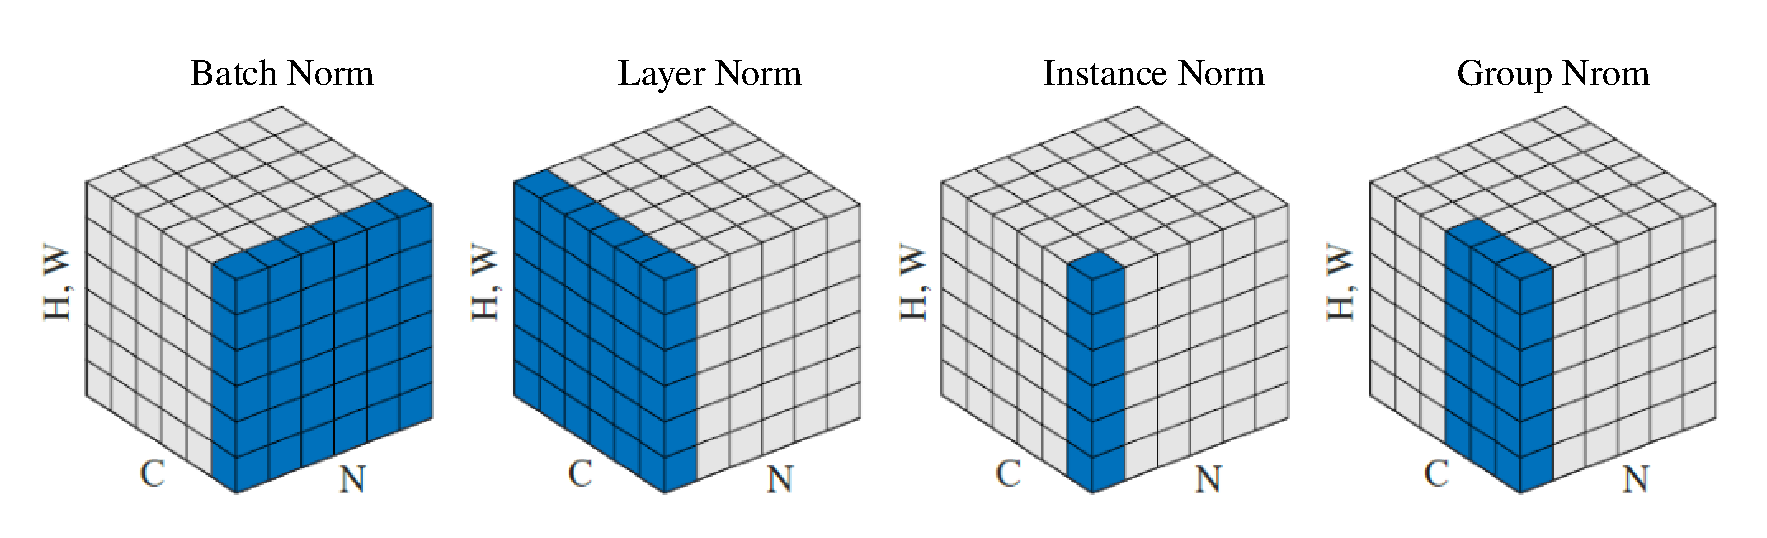
\includegraphics[width=1.0\columnwidth]{norm.pdf}
  \caption{\footnotesize 归一化方法。每一个子图显示的是一个feature map,其中N为batch轴,C为channel轴,(H,W)为空间轴。蓝色的像素表示归一化的范围。}
  \label{fig:norm}
\end{figure}

随着神经网络的规模不断变大,结构的复杂度增加,神经网络越来越难以训练,同时神经网络越来越容易出现过拟合的现象。归一化层(normalization layer)成为神经网络中不可或缺的一个层,它能够加快神经网络的收敛速度,防止过拟合,降低神经网络对初始化权重的敏感度,提高神经网络的精度。近几年出现了各种各样的归一化方法,主要包括LRN(Local Response Normalization)~\cite{krizhevsky2012imagenet},BN(Batch Normalization)~\cite{ioffe2015batch},LN(layer Normalization)~\cite{ba2016layer},IN(Instance Normalization)~\cite{dmitry2016instance}和GN(Group Normalization)~\cite{wu2018group}等。

LRN是AlexNet等网络中使用的归一化方法,它在每一个像素的小领域范围内进行归一化处理。目前主流的归一化方法则更加注重全局范围内的归一化处理,这些全局归一化的方法能够使得我们在训练神经网络时使用较大的学习率,从而加快神经网络训练速度。如图~\ref{fig:norm}所示,BN选择在batch维度上进行归一化处理;LN选择在channel维度进行归一化处理;IN执行类似BN的计算,但是仅仅在单个样本执行归一化;GN在IN的基础上对多个样本进行归一化。下面主要对BN的计算方法进行简要介绍。

BN的计算公式如下所示:
\begin{gather}
\mu _{\beta} = \frac{1}{N} \sum_{i=1}^{N} a_i \\
\theta _{\beta}^{2} = \frac{1}{N} \sum_{i=1}^{N}(a_i - \mu _{\beta})^{2} \\
\hat{a_i}=\frac{a_i - \mu _{\beta}}{\sqrt{\theta _{\beta}^2 + \epsilon}} \\
b_i = \gamma \hat{a_i} + \beta
\end{gather}

在上述算法中,$m$为batch数,$a_i$是第i个batch的输入数据,$\mu _{\beta}$ 和 $\theta _{\beta}^{2}$分别是N个输入的均值和方差,参数$\epsilon$是批变化常量,参数$\gamma$和$\beta$是训练时需要学习的参数,$b_i$是最后归一化后的输出。

\subsection{激活层}
激活层(activation layer)是神经网络能够解决非线性问题的关键,它弥补了神经网络中线性模型表达能力不足。目前主流的激活函数包括Sigmoid, Tanh, ReLU以及ReLU的变种,如PReLU和RReLU等。

Sigmoid,Tanh和ReLU的函数图如图x所示,公式分别为
\begin{gather}
Sigmoid(x) = \frac{1}{1 + \eu^{-x}} \\
Tanh(x) = \frac{1-\eu^{-2x}}{1+\eu^{-2x}} \\
ReLU(x)=
\begin{cases}
x & \text{if } x > 0, \\
0 & \text{if } x \leq 0
\end{cases}
\end{gather}

Sigmoid函数主要被应用于早期的神经网络中,Sigmoid函数拥有良好的性质,Sigmoid函数的值域范围限制在(0,1)之间,这与概率值的范围是相对应的,这样sigmoid函数就能与一个概率分布联系起来了;同时Sigmoid函数的导数可以由其本身求得$Sigmoid(x)^{'}=Sigmoid(x)(1-Sigmoid(x))$。但是Sigmoid函数也有不少缺点,首先Sigmoid函数的输出并不是以0为中心,这个特性会导致为在后面神经网络的高层处理中收到不是零中心的数据,进而训练时的权值更新产生锯齿晃动。同时Sigmoid函数具有饱和性,容易出现梯度消失的现象,使得神经网络难以训练。

Tanh函数是Sigmoid函数的改进版本,它的收敛速度比Sigmoid函数更快,相比Sigmoid函数,其输出以0为中心,但是仍然存在饱和性而导致梯度消失的问题的。Tanh函数和Sigmoid函数目前主要被用于基于LSTM的RNN架构或者基于GRU的RNN架构中。

ReLU是目前非常流行的激活函数,它是分段线性函数,所有的负值为0,而正值不变,这种操作被称为单侧抑制。单侧抑制使得神经网络中的神经元也具有了稀疏激活性,尤其体现在深度神经网络模型(如CNN)中,当模型增加N层之后,理论上ReLU神经元的激活率将降低2的N次方倍,从而更好地挖掘相关特征,拟合训练数据。同时,ReLU不存在饱和区,因此不存在梯度消失的问题,使得模型的收敛速度维持在一个稳定的状态。\cite{krizhevsky2012imagenet}实验显示ReLU单元比tanh单元具有6倍的收敛速度提升。

\subsection{LSTM}

\begin{figure}[b]
  \centering
  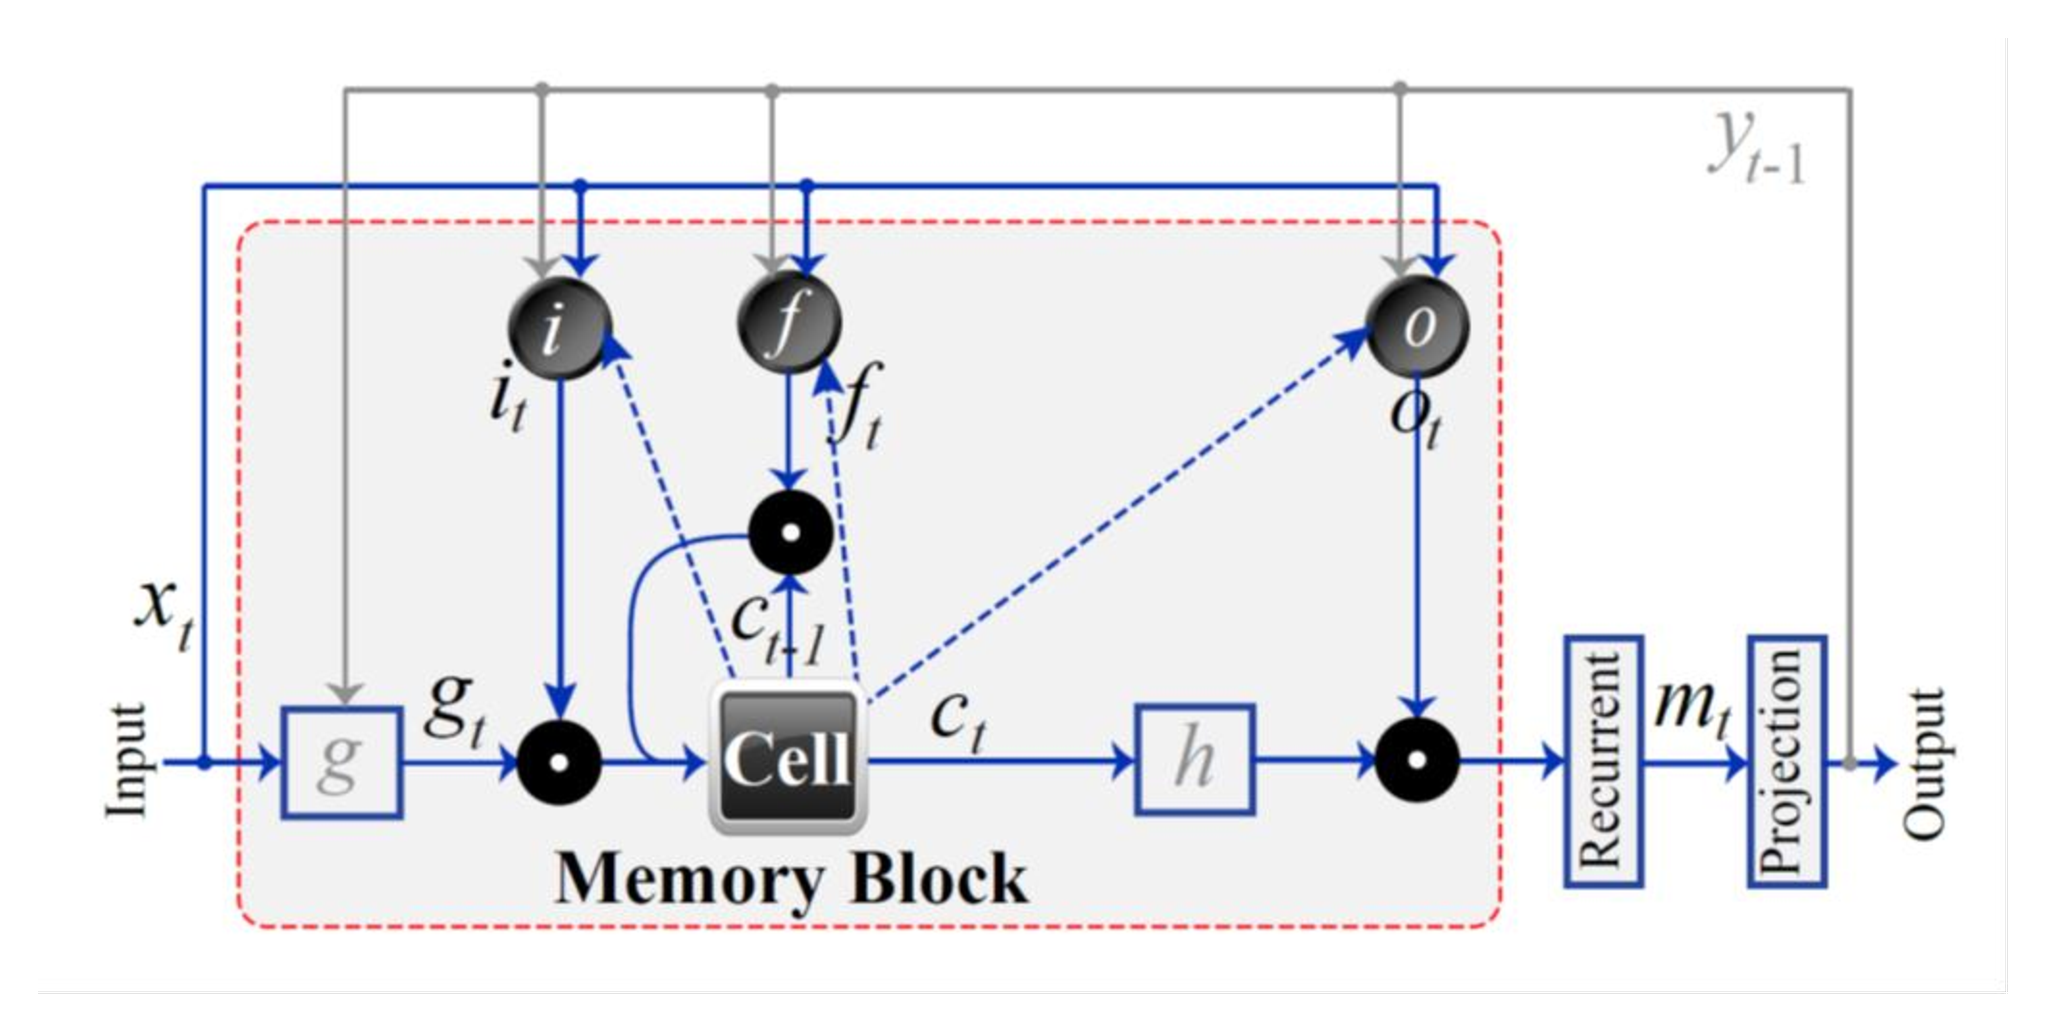
\includegraphics[width=0.7\columnwidth]{lstm.pdf}
  \caption{\footnotesize 一个基于LSTM的RNN架构.}
  \label{fig:lstm}
\end{figure}

\begin{figure}[h]
\centering
\begin{minipage}[b]{0.45\columnwidth}
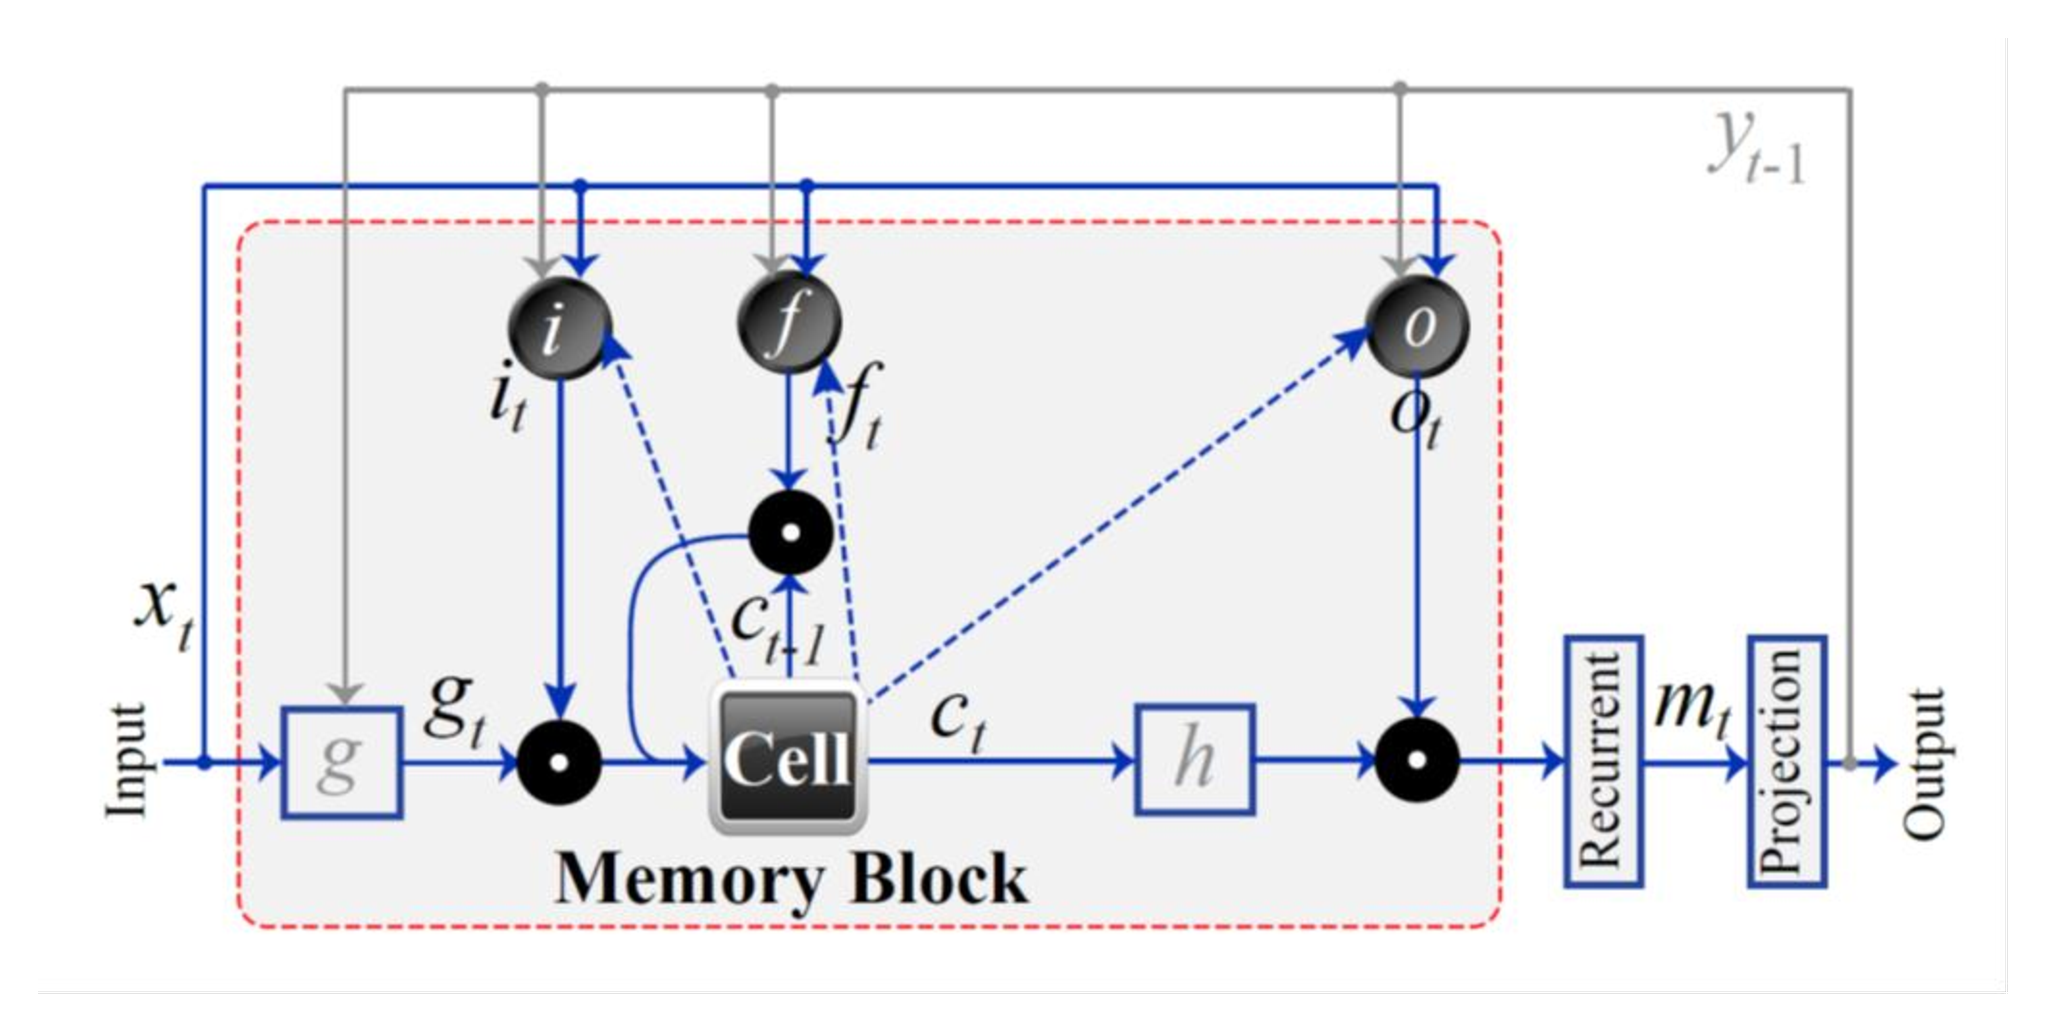
\includegraphics[width=\columnwidth]{lstm.pdf}
\end{minipage}
\hfill
\begin{minipage}[b]{0.45\columnwidth}
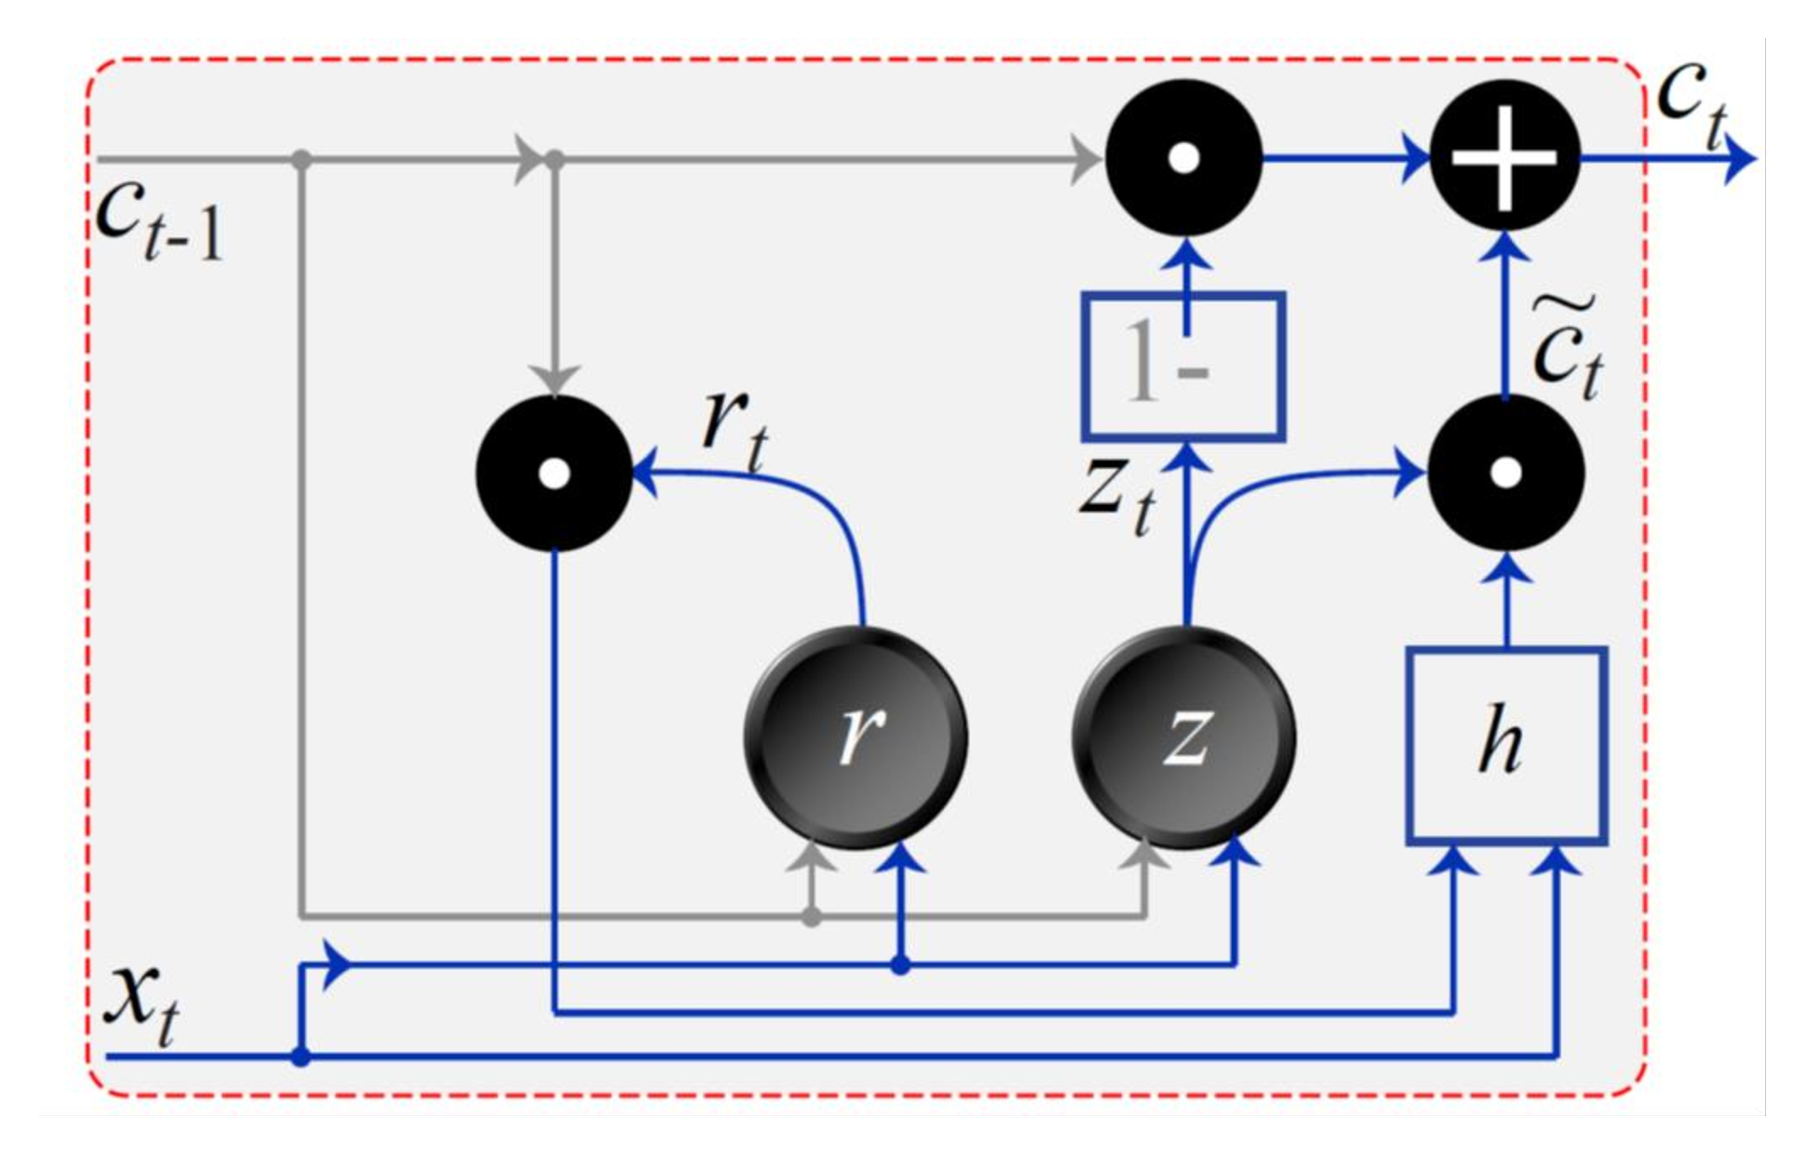
\includegraphics[width=\columnwidth]{gru.pdf}
\end{minipage}
\caption{\footnotesize (a) LSTM (b) A sparse MLP.}
\label{fig:RNN}
\end{figure}

现代大规模自动语音识别(automatic speech recognition,简称ASR)系统利用基于LSTM的RNN作为其声学模型。LSTM模型由一系列大规模矩阵组成,这是ASR的所有步骤中计算量最大的部分。在基于LSTM的RNN中,时刻T的输入取决于时刻T-1的输出。
一个经典的LSTM模型如图~\ref{fig:lstm}所示。
LSTM模型包含特殊存储单元(图~\ref{fig:lstm}中的$cell$)和三个特殊的门(图~\ref{fig:lstm}中的$i$,$o$,$f$),其中$cell$用于存储网络的时间状态信息,门用于执行特殊的乘法运算,包括输入门(input gate)、输出门(output gate)和遗忘门(forget gate)。输入门$i$控制输入到存储单元中的输入量;输出门$o$控制输出值;遗忘门$f$自适应地遗忘$cell$中存储的信息,从而控制前一状态对现状态的影响。除了基本的三个众所周知的门和$cell$之外,该LSTM模型还引入了窥视孔(peephole)和投影层(projection layer),以便更好地学习。窥视孔将缩放后的$cell$状态添加到三个门,其中缩放尺度由三个对角矩阵决定。投影层线性地将输出转换为低维形式。

LSTM模型的接收一个输入序列$X=(x_1;x_2;x_3;...;x_T)$(其中$x_t$是t时刻的输入向量)和上一个状态的输出序列$Y^{T-1}=(y_0;y_1;y_2;...;y_{T-1})i$(其中$y_{t-1}$是t-1时刻的输出向量)。利用下列公式从t=1到T计算输出序列$Y=(y1;y2;y3;...;y_T)$:
\begin{gather}
i_t=\delta (W_{ix}x_t + W_{ir}y_{t-1} + W_{ic}c_{t-1} + b_i), \\
i_t=\delta (W_{ix}x_t + W_{ir}y_{t-1} + W_{ic}c_{t-1} + b_i), \\
f_t=\delta (W_{fx}x_t + W_{fr}y_{t-1} + W_{fc}c_{t-1} + b_f), \\
g_t=\delta (W_{cx}x_t + W_{cr}y_{t-1} + b_c), \\
c_t=f_t \odot c_{t-1} + g_t \odot i_t, \\
o_t=\delta (W_{ox}x_t + W_{or}y_{t-1} + W_{oc}c_{t} + b_o), \\
m_t=o_t \odot h(c_t), \\
y_t=W_{ym}m_t 
\end{gather}

其中符号$i$、$f$、$o$、$c$、$m$和$y$分别是输入门、遗忘门、输出门、$cell$状态、$cell$输出和投影输出;$\odot$表示向量逐元素乘积,$W$表示权值矩阵(例如$W_ix$是从输入向量$X_t$到输入门的权值矩阵),$b$表示偏置向量。值得注意的是$W_ic$、$W_fc$和$W_oc$是用于peephole连接的对角矩阵,因此它们本质上是向量。$\delta$是Sigmoid激活函数,$h$是用户自定义的激活函数,通常情况下会采用$tanh$激活函数。

\subsection{GRU}
\begin{figure}[b]
  \centering
  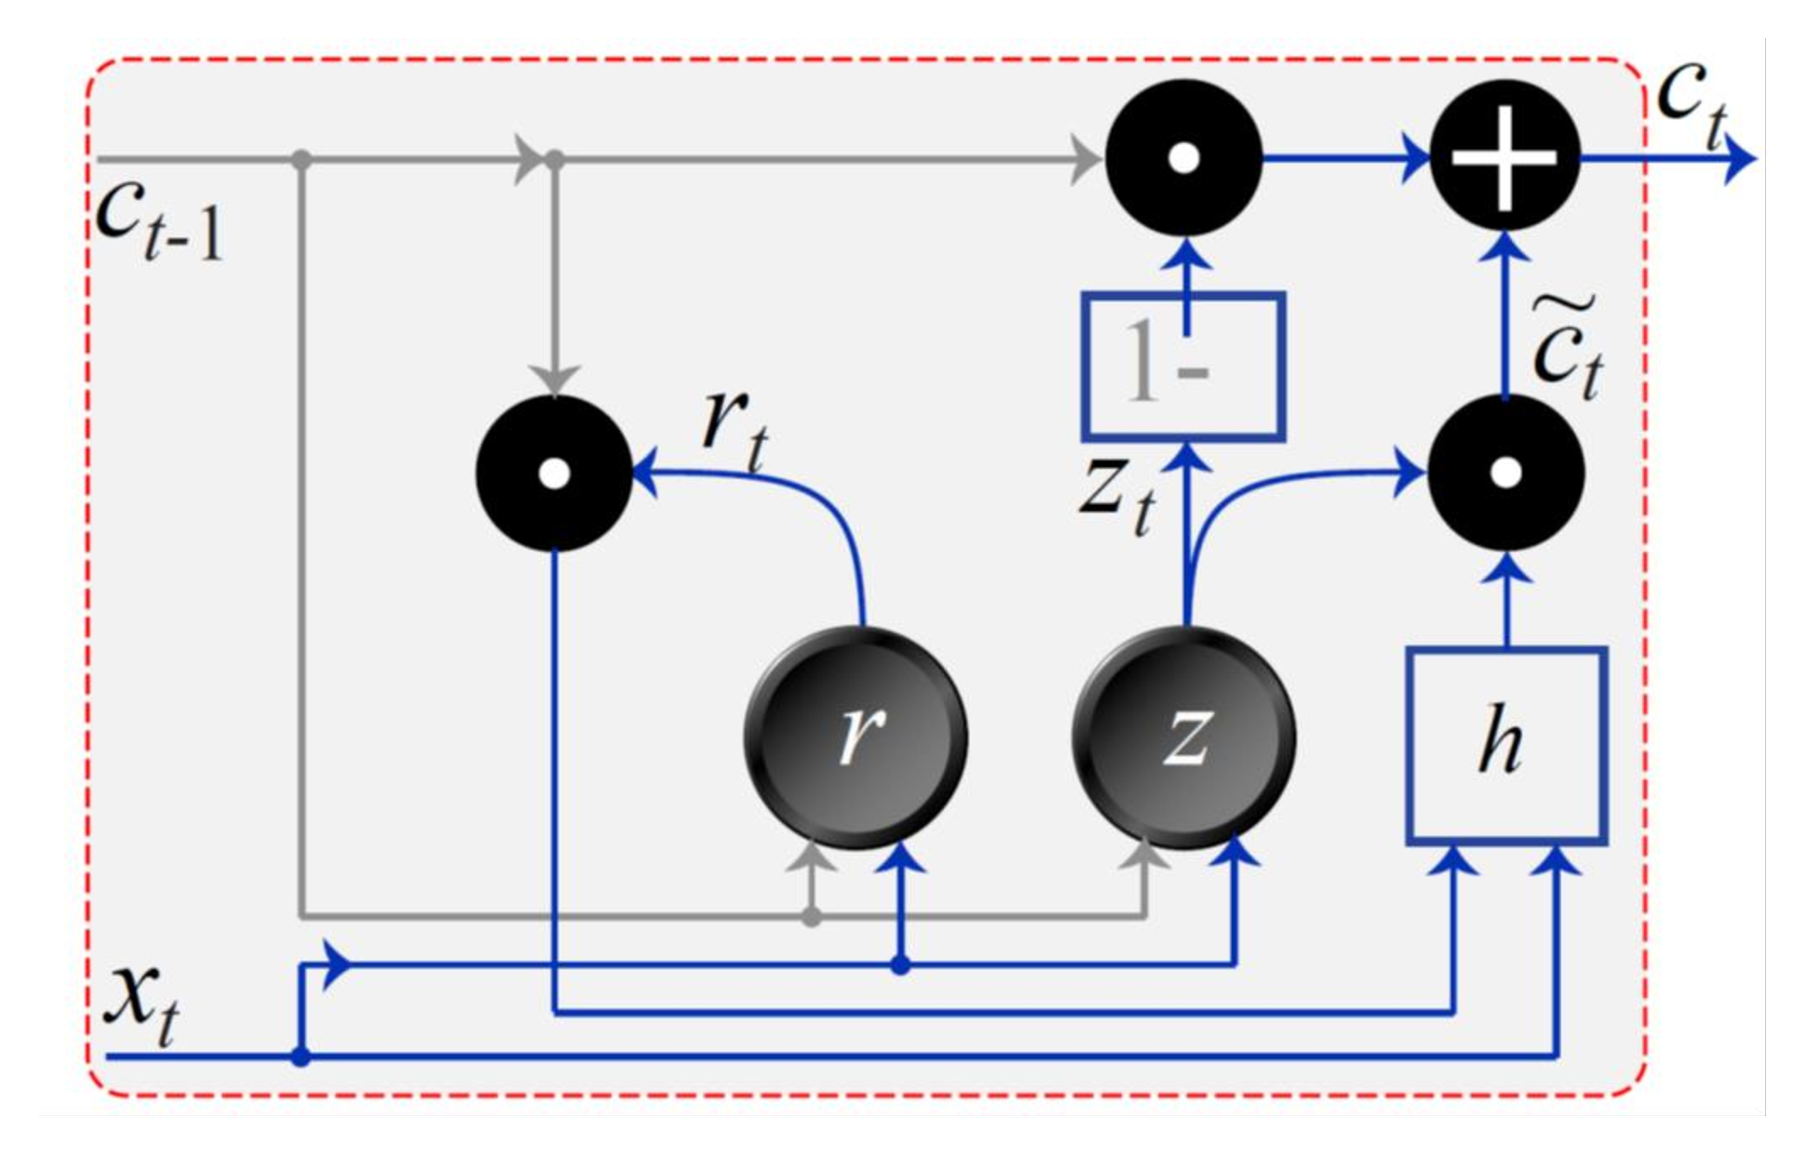
\includegraphics[width=0.7\columnwidth]{gru.pdf}
  \caption{\footnotesize 一个基于GRU的RNN架构.}
  \label{fig:gru}
\end{figure}
GRU是LSTM的变体,它把遗忘门和输入门组合成一个更新门(update gate)。它还合并了$cell$状态和隐藏状态,并进行了一些其他更改。GRU架构如图~\ref{fig:gru}所示。类似地,它遵循如下的公式从t=1到T进行迭代计算:
\begin{gather}
z_t=\delta(W_{zx}x_t+W_{zc}c_{t-1}+b_z),\\
r_t=\delta(W_{rx}x_t+W_{rc}c_{t-1}+b_r),\\
\tilde{c_t}=h(W_{\tilde{c}x}x_t+W_{\tilde{c}c}(r_t \odot c_{t-1}) + b_{\tilde{c}}),\\
c_t=(1-z_t) \odot c_{t-1} + z_t \odot \tilde{c_t}
\end{gather}
其中符号$z$、$r$、$\tilde{c}$、$c$分别是更新门、复位门、复位状态和$cell$状态;$\odot$表示逐元素乘法。$W$表示权值矩阵,$\delta$是Sigmoid激活函数,$h$是用户定义的激活函数,这里我们使用$tanh$激活函数。值得注意的是GRU有两个门(更新门和复位门),而LSTM有三个门(输入门、遗忘门、输出门),GRU中不存在LSTM中存在的输出门,而是将$cell$状态作为输出。LSTM中输入门和遗忘门耦合称为GRU中的更新门$z$,复位门$r$直接作用于到上一个$cell$的状态。 


\section{神经网络低能耗的技术}
随着神经网络算法被应用于更复杂的处理任务和更广泛的场景中,神经网络的规模也越来越大。最新的DNNs~\cite{le2013building, coates2013deep}需要数百兆字节甚至千兆字节来存储神经元和权值;同时需要数十亿次的乘加操作完成运算。考虑未来神经网络将朝着规模更大,层数更深的趋势发展,未来的大规模网络很难部署到嵌入式系统中。因此很多研究人员致力于减少神经网络的参数规模,从而减少存储资源,运算资源和带宽需求,提升性能同时降低能耗。目前已经有了一些有效的算法来解决这个问题,主要方法包括神经网络的低精度计算和神经网络压缩模型。

\subsection{神经网络的低精度计算}

最近研究~\cite{gupta2015deep}表明,在深度神经网络的训练中,不需要全精度的数据。使用低比特的权值表示,可以显著减少网络存储需求和运算能耗,特别是当使用极低比特位,如二进制/三元权值时。研究显示,非精确的计算(在神经元和权重中加入噪音)具有正则化的效果,从而减少泛化误差~\cite{goodfellow2016deep}。~\citet{gupta2015deep}使用16位定点数字表示来训练网络。~\citet{koster2017flexpoint}提出了动态数据格式(FlexPoint),用来完全替代32位浮点格式。Flexpoint具有一个可动态调整的共享指数,以最小化溢出和最大化可用动态范围。在训练过程中,数据范围会随着训练轮数的增长而连续变化,其中共享指数部分可以根据历史数据进行预测。实验结果显示,采用16位尾数和5位共享指数的Flexpoint格式数据在训练神经网络时,能够获得32位浮点类似的精度,并且远远超过16位浮点获得的精度。~\citet{dettmers20158}使用8比特量化神经网络,在保持性能的情况下,加快神经网络训练速度。在~\cite{courbariaux2015binaryconnect}和~\cite{hu2018hashing}中,作者表明,深度神经网络可以通过二进制权值进行训练,在某些情况下,它的精度可能超过使用浮点数进行训练的结果。~\citet{rastegari2016xnor}首先提出了三元权值网络 (Ternary Weight Network, TWN), 并在ImageNet~\cite{russakovsky2015imagenet}数据集上取得良好的效果。三元权值网络在~\cite{li2016ternary,zhu2016trained}等工作中被不断深入研究,其中~\cite{zhu2016trained}提出了学习三元值和三元赋值的方法。~\citet{zhou2017incremental}提出了INQ (Incremental Network Quantization),在不降低网络精度的情况下,将神经网络的权值量化为$2^{-n}$的形式。~\citet{wang2017fixed}提出了定点分解网络 (Fixed-point Factorized Network, FFN),使用定点分解的方式对神经网络权值进行三元化。这些方法可以在ImageNet上达到与全精度相当的精度,但是,这些工作只对权值进行量化,而使激活保持浮点格式。

除了对神经网络权值进行量化外,也有许多研究对激活进行量化。通过将权重和激活转换为低比特格式,网络计算需要使用定点操作,从而更有效地节约资源。~\citet{hubara2016binarized}中提出的二值神经网络 (binarized neural network, BNN),在CIFAR-10这样的小数据集上达到了跟浮点数类似的精度。~\citet{rastegari2016xnor}提出了另一个名为xnorn-net的网络,该网络将权值和激活都进行了二值化,在像ImageNet这样的大数据集上,xnor-net比BNN更精确,但是,它的精度对比浮点数的情况仍然有很大的下降。~\citet{zhou2016dorefa}提出了doref-net,研究了量化时比特位长度对权值、激活和梯度的影响。~\citet{cai2017deep}提出了HWGQ (Half-wave Gaussian Quantization) 的方法对权值和激活同时进行量化。与权值量化相比,激活量化通常会导致更大幅度的精度下降。对AlexNet和VGG16这样的大型网络进行量化,这些方法会导致精确度下降$5\%  ~ 10\%$。因此,如何用低比特位来量化权值和激活仍然是一个具有挑战性的问题。


\subsection{神经网络压缩模型}
大规模的神经网络通常是过拟合的,过多的参数会严重影响神经网络的运算速度。因此,我们可以通过压缩神经网络模型的方式来缓解过拟合的情况,同时减少神经网络的存储需求和运算需求。神经网络压缩的方法可以分为两类,剪枝和矩阵分解。

\citet{han2015learning}提出了剪枝的策略来减少神经网络中权值的数量,在不影响神经网络准确性的前提下,能够将神经网络所需要的存储量和计算量减少一个数量级。剪枝策略首先对神经网络进行训练,找出那些重要的连接;接下来,修剪那些不必要的连接;最后对神经网络进行冲训练,微调剩余连接的权值。实验显示,剪枝策略能够将AlexNet网络的权值数量减少9倍,将VGG16网络的权值数量减少13倍。

在此基础上,~\citet{han2016eie}进一步提出了Deep Compression用来深度压缩神经网络。Deep Comression由三个阶段组成:剪枝(Pruning),量化(quantization)和霍夫曼编码(Huffman Coding),最终在不影响神经网络的精度的前提下将神经网络压缩了35倍到49倍。Deep Compression首先通过剪枝阶段学习网络中重要的连接,删除不必要的连接,这个步骤能够减少9倍到13倍的权值。然后通过聚类算法将权值进行聚类,然后量化权值实现权值的共享,这个步骤能够减少表示每个权值的比特数,从32比特减少到到5比特。最后采用霍夫曼编码进一步无损压缩神经网络,这个步骤能够节省$20\%~30\%$的网络存储开销。在ImageNet数据集上,Deep Compression能够将AlexNet网络压缩35倍,将网络规模从$240MB$压缩到$6.9MB$。同时,Deep Compression将VGG16网络压缩了49倍,将网络规模从552MB压缩到11.3MB。这将允许我们将网络模型存储在加速器的片上SRAM缓存中,而不需要在片上和片外之间反复搬运权值,从而减少片外访存开销。

\citet{wang2016cnnpack}提出了一种新的有效的CNN压缩方法CNNpack,它在频域对神经网络进行剪枝操作,因此它不仅能够关注小的权值,同时关注所有潜在的对计算结果影响小的连接。CNNpack借助离散余弦变换(Discrete Cosine Transform,DCT)将空间域的权值变换到频域,然后采用聚类的方法将频域中的权重分解为公共部分和私有部分(残差)。在这两部分中,采用剪枝的策略丢弃大量的低能级的频率系数,能够在不显著降低精度的情况下产生高压缩比。在此基础上,CNNpack接着采用量化,霍夫曼编码和CSR存储的方法进一步压缩神经网络。最终实验实验显示,CNNpack能够对AlexNet和VGG16分别压缩35倍和49倍。

除了以上对权值进行剪枝的策略,还有不少研究工作直接对神经元进行剪枝操作~\cite{he2014reshaping,srinivas2015data,hu2016network,mariet2015diversity}。但是对神经元直接进行剪枝操作会严重降低神经网络的精度,因此不能获得很低的稀疏度。Data-free Parameter Pruning~\cite{srinivas2015data}在AlexNet和LeNet5上仅仅能够获得$65.11\%$和$16.5\%$的稀疏度,远远高于权值剪枝策略~\cite{han2015learning}的$11\%$和$8\%$。Network Trimming~\cite{hu2016network}能够在VGG16和LeNet5上获得$37\%$和$26\%$的系数率,也高于~\cite{han2015learning}中的$7.5\%$和$8\%$。

除了经典的剪枝策略(包括权值剪枝和神经元剪枝),还有一部分的研究工作基于矩阵分解和因式分解~\cite{denton2014exploiting,jaderberg2014speeding,lebedev2014speeding},这些方法可以保持原始模型的规则密集计算结构,在通用处理器上实现神经网络压缩和加速。~\citet{denton2014exploiting}是利用神经网路线性结构的特性,对神经网络进行适当的低秩分解(low-rank approximation),在精度损失在$1\%$的情况下,在很多模型上都能获得超过2倍的加速。~\citet{jaderberg2014speeding}利用将$k\times k$的卷积核分解为$k\times 1$和$1\times k$的卷积核,从而加速卷积计算。同时~\cite{jaderberg2014speeding}提出了两种优化方案:一种是利用滤波重构的方法最小化滤波权值误差,另一种是利用数据重构最小化响应误差的。~\citet{lebedev2014speeding}则采用CP decomposition的方式对大规模神经网络的卷积核进行分解和加速,实验结果显示,在精度损失低于$1\%$的情况下,在AlexNet网络能够获得4倍的加速效果。



\section{神经网络加速器}
\begin{table}[b]
  \footnotesize
  %\small
  \centering
\caption{\footnotesize 现有神经网络加速器的数据流形式}
\label{tab:dataflow}
\begin{tabular}{@{}lllll@{}llllllll}
  \toprule
  数据流 & 加速器\\
  \midrule
  基于向量算子的数据流 & DianNao~\cite{chen2014diannao}, DaDianNao~\cite{chen2014dadiannao}, PuDianNao~\cite{liu2015pudiannao}, Cambricon~\cite{liu2016cambricon}, \\ 
  ~ & Cambricon-X~\cite{zhang2016cambricon}, Cnvlutin~\cite{albericio2016cnvlutin}, EIE~\cite{han2016eie}, ESE~\cite{han2017ese} \\
  基于乘加算子的空间数据流 & ShiDianNao~\cite{du2015shidiannao}, Eyeriss~\cite{chen2017eyeriss}, TPU~\cite{jouppi2017tpu}, Neuflow~\cite{farabet2011neuflow} \\
  ~& SCNN~\cite{angshuman2017scnn}  \\
\bottomrule
\end{tabular}
\end{table}

\begin{figure}[t]
  \centering
  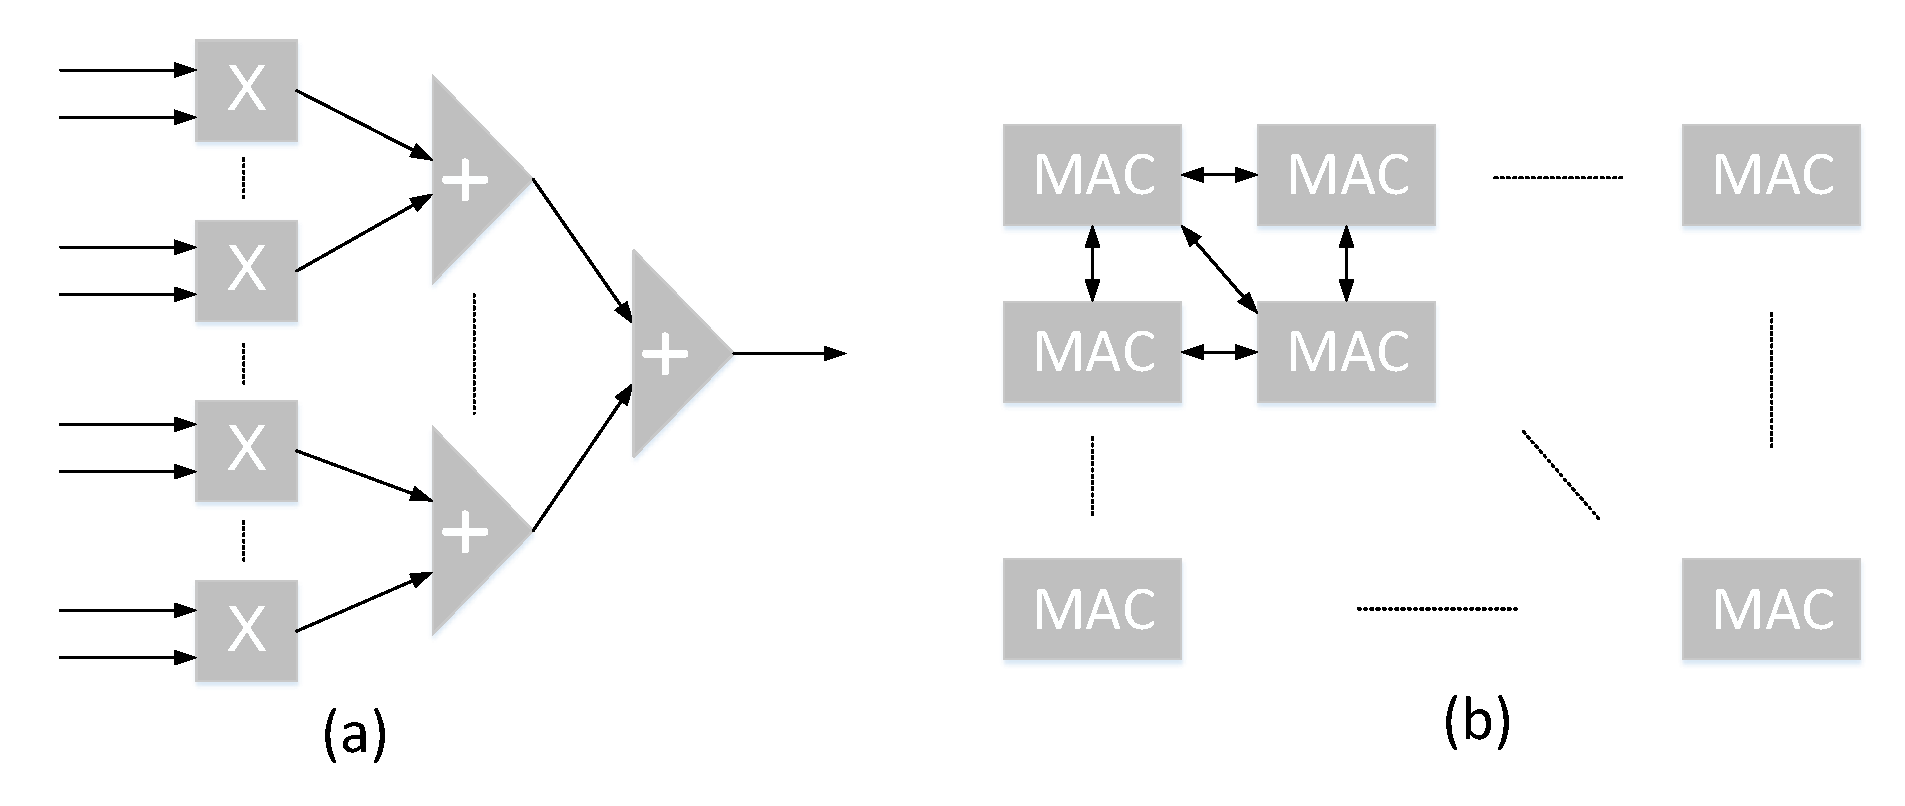
\includegraphics[width=0.7\columnwidth]{dataflow.pdf}
  \caption{\footnotesize 现有的加速器架构.}
  \label{fig:dataflow}
\end{figure}

\subsection{现有神经网络加速器架构}
由于严峻的能耗约束和高性能要求,定制加速器成为CPU和GPU等传统处理平台的替代品。近几年出现了数据流和结构各异的神经网络加速器。神经网络加速器按照数据流的形式可以分为两类,分别是基于向量算子数据流的加速器和和基于乘加算子(multiply-and-accumulate,简称MAC)空间数据流的加速器。基于向量算子的加速器将神经网络的运算转化为向量运算,主要是将矩阵操作转化为一系列的向量操作(通常是内积操作)。如图~\ref{fig:dataflow} (a) 所示的结构中,n个乘法器和一个n输入的加法树就能够完成两个n维向量的内积操作。基于乘加算子的加速器(如图~\ref{fig:dataflow}(b))通常具有一系列的规则分布的处理单元,其中每一个处理单元能够完成一次MAC操作。处理单元之间采用一种规律的方式进行连接(如二维矩阵),神经元和权值采用某种规律的方式在处理单元之间进行移动,如经典的脉动阵列形式(systolic design),因此这种形式又称为空间数据流形式。表~\ref{tab:dataflow}总结了近年来出现的神经网络加速器和它们的数据流形式。
基于向量算子的神经网络加速器包括DianNao~\cite{chen2014diannao},DaDianNao~\cite{chen2014dadiannao},PuDianNao~\cite{liu2015pudiannao},Cambricon~\cite{liu2016cambricon},Cambricon-X~\cite{zhang2016cambricon},Cnvlutin~\cite{albericio2016cnvlutin}, EIE~\cite{han2016eie}和ESE~\cite{han2017ese}。基于乘加算子空间数据流的加速器包括ShiDianNao~\cite{du2015shidiannao}, Eyeriss~\cite{chen2017eyeriss}, TPU~\cite{jouppi2017tpu}, Neuflow~\cite{farabet2011neuflow}和SCNN~\cite{angshuman2017scnn}。


\begin{figure}[t]
  \centering
  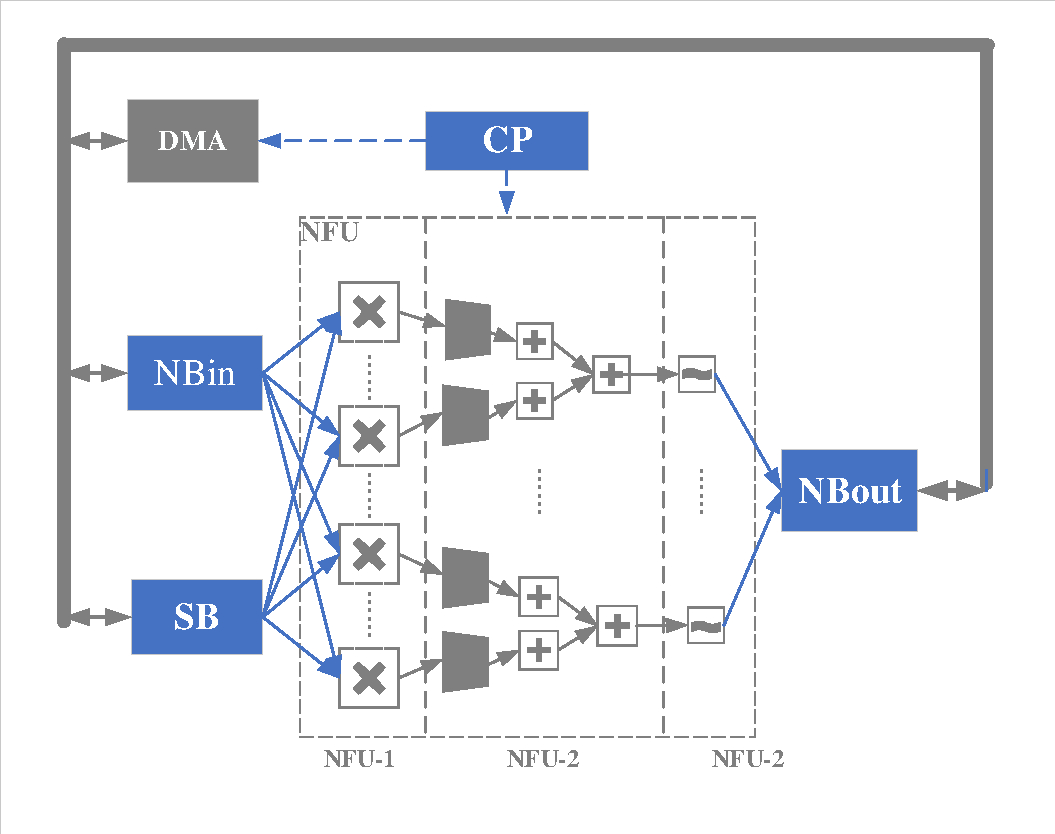
\includegraphics[width=1.0\columnwidth]{diannao.pdf}
  \caption{\footnotesize (a)DianNao加速器结构。(b)DaDianNao一个tile的结构。 (c)DaDianNao一个node的结构}
  \label{fig:diannao}
\end{figure}

\subsection{基于向量算子的神经网络处理器}
DianNao是世界上首个深度神经网络处理器,它的结构如图~\ref{fig:diannao}所示。DianNao包含以下的主要模块:一个控制器(Control Processor,简称CP),一个神经功能单元(Neural Functional Unit, 简称NFU),三个片上缓存(NBin,NBout和SB)和外部存储接口(Memory Interface)。CP采用自定义的指令控制DianNao的运行。NBin,NBout和SB分别用来缓存输入神经元,输出神经元和权值。NFU包含$T_n$个计算单元,每个计算单元包含$T_n$个乘法器和一个$T_n$输入的加法树。在计算过程中每个计算单元共享输入神经元,接收不同的权值,从而计算不同的输出神经元。因此NFU最多读取$T_n$个输入神经元,$T_nxT_n$个权值,计算$T_n$个输出神经元。在TSMC65nm工艺下,采用$T_n$=16的配置,DianNao的面积,功耗和吞吐率分别为$3.02mm^2$,$485mW$和$452GOP/s$,对比与一个2GHz的CPU,能够获得117倍的性能提升,并且降低21倍的能耗。

DadianNao是DianNao的多核版本,一个NFU与外围的存储模块构成一个tile,多个tile通过fat-tree进行局部互联组成一个node,最终多个node通过HyperTransport2.0互联形成DaDianNao。DaDianNao使用eDRAM来提供足够的片上缓存用来存储权值和神经元,从而减少片外访存开销,进而有效地处理大规模神经网络。实验显示,在ST28nm的工艺下,64核的DaDianNao的面积和功耗分别是$67.73mm^2$和$15.97W$,对比Nvidia K20,平均性能提升21.38倍,平均能耗降低了330.56倍。

PuDianNao是一个机器学习处理器,它不仅支持神经网络算法,而且支持K最近邻算法(K-Nearest Neighbors,简称K-NN),K均值算法(K-Means),线性回归(Liner Regression,简称LR),支持向量机(Support Vector Machine,简称SVM),朴素贝叶斯(Naive Bayes,简称NB)和决策树(Classification Tree,简称CT)等多种机器学习算法。PuDianNao深入分析上述机器学习算法,并且提取出机器学习中的核心运算,其中包括向量内积(LR、SVM和DNN),距离计算(K-NN和K-Means),计数(CT和NB),排序(K-NN和K-Means),非线性函数(如sigmoid和tanh)等。PuDianNao的核心模块是机器学习单元(Machine Learning Unit,简称MLU),如图x所示,MLU包括六个流水级,分别为Counter,Adder,Multiplier,Adder Tree,Acc和Misc,通过这六个流水级的组合,PuDianNao能够完成机器学习的核心运算。实验显示,在65nm的共一下,PuDianNao的面积和功耗分别为$3.51mm^2$和$596mW$分为对比NVIDIA K20能够提高1.2倍的性能并且减少129.41倍的能耗。

然而随着神经网络算法的飞速发展,一些新的层类型和新的操作不断涌现,如ROI Pooling层,Deconvolution层等,这又迫使研究者开发新的加速器和指令集来支持这些新的层和操作。为了进一步提高神经网络加速器的通用性,Liu等人提出了针对神经网络处理器的指令集Cambricon。Cambricon的主要思想是为神经网络加速器提供一系列的基本算子(即指令),然后通过这些基本算子逐步搭建完成神经网络的运算。Cambricon中集成了控制,数据传输,运算和逻辑操作这四种不同的指令,其中运算指令进一步分为矩阵运算,向量运算和标量运算指令,研究者只需要基本指令就能完成神经网络的运算。基于Cambricon指令集设计的加速器能够比DaDianNao拥有更强的通用性,在10个benchmark中,DaDianNao只能支持其中的三种,而基于Cambricon的加速器能够全部支持。同时对比与Intel Xeon E5-2620和NVIDIA K40,加速器能够分别获得91.72倍和3.09倍的性能提升。

\subsection{基于乘加算子空间数据流的神经网络处理器}
ShiDianNao是面向嵌入式设备的神经网络处理器,实现端到端的神经网络应用。ShiDianNao的架构如图x所示,ShiDianNao与DianNao最大的不同是NFU模块。ShiDianNao的NFU是一个大小为$P_x\times P_y$的二维处理单元阵列(Processing Elements, 简称PEs),它采用脉动阵列的形式完成神经网络矩阵向量运算操作。每个PE在每个周期能够完成卷积层、全连接层的一次乘法和一次加法,或者平均池化层的一次加法或者最大池化层的比较操作。每个PE能够从右方邻居和下方邻居读取神经元,并且能将部分和传播给相邻的PE,值得注意的是权值通过广播的形式传送给PE。这种方法能够充分复用神经元和权值,从而提高性能并降低访存能耗。在$P_x=P_y=8$的配置下使用65nm工艺,ShiDianNao的主频,面积和功耗分别为$1GHz$,$4.86mm^2$和$320.1mW$,对比GPU和DianNao能够分别获得30倍和1.87倍的加速比,减少4700倍和60倍的能耗。除了ShiDianNao,Farabet等人提出的Neuflow,Chen等人提出的Eyeriss和谷歌的TPU(tensor processing unit)均采用二维网格的形式排列处理单元,并且采用脉动阵列的形式完成神经网络运算。其中Google的TPU主要用来加速其第二代人工智能系统TensorFolow的运行,并且相比于K80能够有15倍的性能提升。


\subsection{稀疏神经网络处理器}
虽然上述加速器能够以低能耗实现高吞吐量,但它们不能利用现代压缩神经网络的稀疏性和不规则性。最近出现了一些能够支持稀疏的神经网络加速器~\cite{chen2017eyeriss,zhang2016cambricon,albericio2016cnvlutin,han2016eie,han2017ese,angshuman2017scnn}
,但它们都有各自的优缺点,如表~\ref{tab:comp}所示。

Eyeriss~\cite{chen2017eyeriss}应用游程压缩方法(run-length-compression,RLC)对稀疏神经元进行编码,具体来说,它在架构中加入RLC Encoder对输出神经元进行压缩,同时采用RLC Decoder对输入神经元进行解压缩,从而减少访问DRAM的数据量,进而减少DRAM的带宽需求和访存能耗。同时Eyeriss在PE单元中加入控制门,当输入神经元为0时,PE单元将被关闭,这样能够跳过不必要的计算,从而减少计算能耗。然而,这两种方法仅仅能够带来能耗的减少,不会带来性能增益。

Cambricon-X~\cite{zhang2016cambricon}能够充分挖掘稀疏权值带来的收益,包括减少能耗和提升性能。Cambricon-X使用步长索引的形式压缩静态的权值,从而减少片外和片上访存能耗开销。同时Cambricon-X利用索引模块(indexing module,IM)来挖掘稀疏的特性,IM能够通过稀疏的权值位置信息过滤掉不需要参与计算的神经元。IM模块的结构如图x所示,首先,IM模块连续地累加权值索引表的值(也就是图中的 1132),这些累加后的值就是每个连接相对起始点的位置,然后采用MUX的逻辑就能选出与非零权值对应的神经元(即n1,n2,n5,n7)。Cambricon-X对比不支持稀疏特性的DianNao提高了7.23倍的性能,并减少了6.43倍的能耗,但是Cambricon-X并不能挖掘稀疏神经元带来的收益。

Cnvlutin~\cite{albericio2016cnvlutin}能够利用动态神经元稀疏筛选出需要进行计算的权值,从而获得1.37倍的加速比,但是Cnvlutin不能利用权值稀疏特性。ESE~\cite{han2017ese}是实现在FPGA上的加速器,它面向的是稀疏的LSTM模型,并不适用于稀疏的CNN模型;由于LSTM模型中使用Tanh作为激活函数,因此不存在神经元稀疏的特性,所以ESE仅仅能够挖掘权值稀疏的特性。

以上工作只能挖掘权值稀疏性或者神经元稀疏性,但不能同时从两者中受益。EIE~\cite{han2016eie}采用稀疏矩阵的行压缩形式(compressed sparse row,简称CSR)存储稀疏的权值,并且通过LZND(leading non-zero detection)筛选出非零的神经元,使得使得EIE能够同时利用神经元稀疏性和权值稀疏性,对比与DaDianNao能够提高2.9倍的性能,减少19倍的能耗并且缩小3倍的面积。但是这种架构仅仅针对全连接层的计算,并不能针对卷积层进行计算。

SCNN~\cite{angshuman2017scnn}能够同时利用神经元稀疏性和权值稀疏性。SCNN中的计算单元构成了一个二维网格的形式,每个计算单元执行非零神经元和非零权值的乘法操作,同时计算非零乘积的坐标。非零乘积通过坐标在二维计算网络进行路由,最终被分配给对应的累加器阵列,每个非零乘积通过读取修改写入操作对包含部分和的本地RAM执行累加,最终获得输出神经元。但是这种架构需要不断计算坐标,大大增加了计算成本和存储成本。因此SCNN在处理稠密神经网络时的会损失$21\%$的性能,同时增加$33\%$的能耗;在处理稀疏神经网络时仅仅能够增加2.7倍的性能,减少2.3倍的能耗。同时SCNN对全连接层和规模为1x1的卷积层支持并不理想,在这两种类型的层时时只能利用$20\%$的乘法器资源。
 
